% -*- mode: LaTeX; coding: utf-8; -*-

\chapter{Katsaus yleisimpiin hyökkäyksiin}

\section{Yleistä}

Nykyisin yksikään verkossa oleva kone ei ole suojassa tietoturvahyökkäyksiltä
ja niiden tuomilta ongelmilta. Useimmat hyökkäykset ovat hyvin monimuotoisia, ja
ne voidaan jakaa eri kategorioihin niiden tavoitteiden ja toteutustapojen
mukaan. Uusia hyökkäystapoja kehitetään jatkuvasti lisää, ja vanhat saavat uusia
ominaisuuksia. Vaikka osaan hyökkäyksistä on olemassa erilaisia suojautumistapoja, 
on näiltä kaikilta suojautuminen ylläpitäjän kannalta mahdoton tehtävä. Verkon
turvallisuuden kannalta on kuitenkin tärkeää, että niiden tuomat riskit
tiedostetaan, ja niihin pyritään puuttumaan  mahdollisuuksien ja resurssien
mukaan.

\section{Tiedon urkinta ja väärentäminen}

Ennen kuin hyökkääjä pystyy murtautumaan verkkoon tai koneeseen, tulee hänen
selvittää kohteen mahdolliset heikkoudet. Haluttuja tietoja ovat mm. mitä
käyttöjärjestelmiä koneisiin on asennettu, mitkä versiot ohjelmistoista on
käytössä ja mikä on verkon rakenne ja tietoturvataso. Näiden tietojen
selvittämiseksi hyökkääjää aloittaa verkkoa kohtaan joukon hyökkäyksiä, joita
kutsutaan tiedusteluhyökkäyksiksi (engl. Probe Attacks). Kyseiset hyökkäykset
ovat hyökkäyksistä yleisimpiä, sillä niiden toteuttaminen ei vaadi hyökkääjältä
kovinkaan syvällistä osaamista. Verkosta löytyy paljon valmiita työkaluja,
joiden avulla hyökkääjä pystyy urkkimaan tarvittavat tiedot, sekä mahdollisesti
saman tien hyödyntämään löydettyjä heikkouksia. Hyökkääjä, jolla on tarkka
kuvaus verkon laitteista ja palveluista, voikin käyttää tietoa
haavoittuvuuksien etsimiseen ja järjestelmiin murtautumiseen \cite{IDS}.

Kun hyökkääjällä on tietämys verkon eri komponenteista, voi hän aloittaa
hyökkäyksen suunnittelun. Yksi tapa murtautua IP-pohjaiseen verkkoon
on hyödyntää protokollissa olevia heikkouksia. Tällaisia hyökkäyksiä kutsutaan
spoofing- eli kalasteluhyökkäyksiksi, ja niissä murtautuja pyrkii naamioimaan oman koneensa
siten, että se näyttäa kuuluvan kohteena olevan koneen kanssa samaan verkkoon.
Tällöin hyökkääjä pystyy huijaamaan kohdekonetta jakamaan ja lähettämään
arkaluontoista tietoa, jota jaettaisiin muuten vain luotettavien osapuolien kesken.
Tällaiset hyökkäyset jaotellaan sokeisiin tai aktiivisiin hyökkäyksiin sen mukaan, 
kuinka paljon tietoa hyökkääjällä on verkosta. Sokeassa hyökkäyksessä kohdekoneen
lähettämiä vastauksia ei pystytä seuraamaan, koska usein murtautujan oikeudet ovat puutteellisia
ja koneen käyttämä IP, joksi hyökkääjä haluaa naamioitua, on harvoin tiedossa.
Aktiivisessa hyökkäyksessä murtautujalla taas on tieto koneiden välisistä oikeuksista,
jolloin tiedon korruptoiminen, muokkaaminen ja välittäminen toiseen verkkoon
on helppo toteuttaa \cite{WEBS}.

\subsection{IP Spoofing}

IP Spoofing on hyökkäystapa, jossa pyritään murtautumaan verkkoon ja hankkimaan
arkaluontoista tietoa väärentämällä lähetettäviin paketteihin luotetun koneen
IP-osoite. Hyökkäykset jaotellaan sokeisiin ja aktiivisiin hyökkäyksiin sen mukaan,
mistä hyökkäys toteutetaan. Hyökkäykset toimivat siten, että kolmivaiheisen yhteydenmuodostuksen aikana
hyökkääjä tekeytyy koneeksi, johon halutulla kohteella on luottamussuhde. Tämä tapahtuu
muokkaamalla lähetettävien pakettien otsaketietoja ja kuittausnumeroita. Tässä onnistuakseen
hyökkääjän tulee pystyä vastaamaan oikeilla kuittausnumeroilla kohteen lähettämiin
paketteihin. Nämä kuittausnumerot hyökkääjä joutuu aluksi usein arvaamaan, jonka takia tämä
hyökkäystapa on vaikea toteuttaa \cite{WEBS}. Niin kutsuttu ``Man in The Middle'' hyökkäys, jossa hyökkääjä 
kaappaa kahden koneen välisen yhteyden, perustuu myös IP-osoitteen väärinkäyttöön (kuva \ref{Man}).

\begin{figure}[ht]
\centering
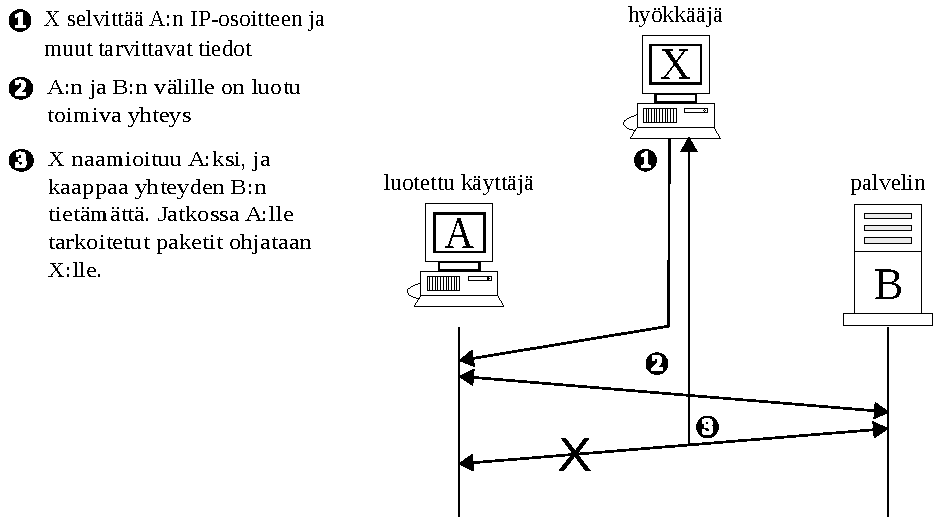
\includegraphics[width=13cm]{pics/MiTM.pdf}
\caption{Man in The Middle-hyökkäys}
\label{Man}
\end{figure}

Vaikka IP-osoitteen varastamiseen perustuvat hyökkäykset ovat vaikeita toteuttaa,
ovat ne melko yleisiä, koska jokainen TCP/IP protokollaa käyttävä järjestelmä on sille altis. Tämä
johtuu siitä, että TCP/IP-pino sallii pakettien käsin muokkaamisen. Tämä
toiminto on sallittu, koska toimiakseen jotkut IP-pohjaiset palvelut joutuvat
käsin muokkaamaan pakettien sisältöä ennen lähettämistä. Tällaisia palveluita
ovat mm. mobiili IP-ympäristö ja VPN-järjestelmät, joissa lähettäjän IP
muutetaan toiseksi \cite{DDOS}.

IP spoofing hyökkäyksiä voidaan torjua monin eri keinoin. Tehokkain tapa on
määrittää verkko siten, että se ei salli sellaisten pakettien kulkua, jotka
väittävät kuuluvansa sisäverkon koneelle, mutta jotka tulevat verkkoon
ulkopuolisista liitännöistä. Jos tämä kuitenkin halutaan sallia, niin jokainen
sessio tulisi kryptata reitittimessä. Muutenkin yhteyksien muodostumisen tulisi
pohjautua koko järjestelmän kattavaan salaukseen \cite{WEBS}.

\subsection{ARP Spoofing}

Nykyisin lähes jokainen verkko pohjautuu TCP/IP-protokollan ja Ethernet-verkon
väliseen toimintaan. Tämän toiminnan mahdollistamiseksi tarvitaan ARP-pro\-to\-kol\-laa,
jonka tehtävänä on selvittää jokaista IP-osoitetta vastaava Ethernet- eli MAC-osoite. Tämä osoite
on uniikki jokaiselle verkkokortille, ja sen avulla verkossa olevat koneet pystytään tunnistamaan.
Tämä tieto tarvitaan, koska ilman sitä verkko ei pysty välittämään paketteja oikealle koneelle.
ARP-spoofing, jota kutsutaan myös ARP-myrkyttämiseksi, pyrkii hyödyntämään ARP-protokollan
toimintaa syöttämällä reitittimissä ylläpidettäviin ARP-tauluihin virheellistä
tietoa (kuva \ref{ARP-spoofing}). Tämä tapahtuu kaappaamalla verkon yleislähetysviestejä, ja muokkaamalla
kuittausviestien sisältöä siten, että kuittausviesteihin hyökkääjä laittaa
kohdeosoitteeksi oman IP-osoitteen ja vastaa viestiin omalla MAC-osoitteella.
Tämän jälkeen kohdekoneelle tarkoitetut paketit ohjautuvat hyökkääjän koneelle \cite{WEBS}.

\begin{figure}[ht]
\centering
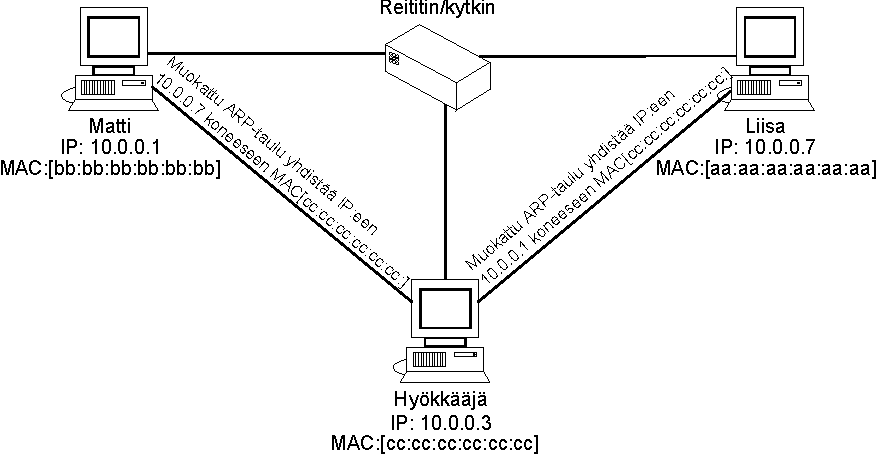
\includegraphics[width=12cm]{pics/arp.pdf}
\caption{ARP-taulun myrkyttäminen käyttäen Man in The Middle hyökkäystä}
\label{ARP-spoofing}
\end{figure}

ARP-protokolla on hyvin haavoittuvainen hyökkäyksille, koska oletuksena se ei
sisällä suojauskeinoa ARP-myrkyttämiselle. Siksi paras keino suojautua
tällaisilta hyökkäyksiltä on varmistaa, että ennen ARP-taulun muokkausta
tunnistetaan käyttäjät jollakin keinolla. Toinen mahdollisuus on käyttää
staattista ARP-taulua \cite{WEBS}.

\section{Denial Of Service}

Yksi tietoturva-alan johtavista tutkimuskeskuksista CERT \cite{CERT}
määrittelee palvelunestohyökkäyksen (engl. Denial of Service)
sellaiseksi teoksi, jossa hyökkääjän tavoitteena on estää laillisia
käyttäjiä käyttämästä heille kuuluvia tai käytössä olevia
palveluita. Tällaisia palveluita voivat olla esimerkiksi verkon
resurssien käyttö sekä verkon yli käytettävät
web-sovellukset. Hyökkäyksillä pyritään lamauttamaan palvelua tarjoava
verkko tai palvelin siten, että oikeiden pyyntöjen vastaanottamiseen
ei enää riitä resursseja. Keinoja tähän on monia, ja koska näistä
lähes jokainen käyttää nykyisin hyväkseen eri protokollien sallittuja
toimintoja, on hyökkäyksiä vastaan suojautuminen hyvin vaikeaa \cite{Hacking}.

Palvelunestohyökkäykset voidaan jakaa kolmeen ryhmään näiden
toteutustapojen ja tavoitteiden mukaisesti. Ensimmäiseen ryhmään kuuluvat
hyökkäykset, joiden tarkoitus on rajoitettujen resurssien loppuun
kuluttaminen. Tämä voidaan toteuttaa esimerkiksi kuormittamalla verkko
tai palvelin turhilla pyynnöillä. Toiseen ryhmään kuuluvat
hyökkäykset, jotka pyrkivät joko tuhoamaan tai muuttamaan
konfigurointitietoja siten, että kone tai verkko ei toimi enää
ollenkaan. Viimeiseen ryhmään kuuluvat verkon komponenttien
muokkaamiseen tai tuhoamiseen tähtäävät hyökkäykset \cite{CERT}. Vaikka tässä
työssä keskitytään vain resursseihin kohdistuviin hyökkäyksiin, niin
palvelun kokonaisturvallisuuden kannalta ylläpitäjän tulee kiinnittää 
jokaiseen ryhmään tasapuolisesti huomiota.

Viime vuosina palvelunestohyökkäykset ovat edelleen kehittyneet
käsittämään verkkokerroksen raa’an voiman hyökkäysten lisäksi myös
sovelluskerroksen hyökkäykset, joiden toteuttaminen vaatii usein
hyökkääjältä vain vähän omia resursseja \cite{Hacking}. Nämä sovelluskerroksen
hyökkäykset ovat toteutukseltaan hyvin hienostuneita, ja ne
jäävät yleensä huomaamatta yrityksen tietoturvaratkaisuilta, koska ne
eivät poikkea normaalista liikenteestä. Hyökkääjä saattaa esimerkiksi
pyytää sellaista resurssia palvelulta, jonka pyytäminen vie vain vähän
hyökkääjän omia resursseja, mutta aiheuttaa palvelimelle suuren
kuorman \cite{DDOSb}. Tällaisen hyökkäyksen teho nähtiin vuonna 2004, kun
MyDoom-viruksella saastuneet koneet kuormittivat yleisimpiä
hakukoneita etsimällä näiden avulla uusia sähköpostiosoitteita, joihin
lähettää saastunut sähköposti \cite{Hacking}. Sovelluskerroksen hyökkäyksen
vaikutus voidaan kohdistaa myös haluttua palvelua kohti, jolloin
vaikutukset ovat vieläkin suuremmat. Näin tapahtui, kun Yhdysvalloissa
yrittäjä palkkasi ”DDoS mafian” kaatamaan kilpailijoidensa nettisivut
HTTP-kutsuilla, jotka pyysivät ladattavaksi isoa kuvatiedostoa
\cite{DDOSb}. Tämä aiheutti kolmelle kilpailijalle arviolta jopa yhden
miljoonan dollarin tappiot, ja pysäytti heidän toimintansa lähes kahdeksi
viikoksi \cite{FBI}.

\subsection{SYN-hukuttaminen}
TCP/IP-protokollan yksi suunnittelulähtökodista oli, että sitä
käytettäisiin avoimessa ja luotetussa ympäristössä. Tästä syystä sen
suunnittelussa ei osattu ottaa huomioon mahdollisia vihamielisiä
käyttäjiä, jotka pyrkisivät häiritsemään muita käyttäjiä sen
avulla. TCP/IP-protokollan käyttö kuitenkin levisi ja yleistyi
arvaamattomasti, jonka johdosta suunnitteluvaiheessa tehdyt virheet
periytyivät nyt käytössä olevaan IPv4-verkkorakenteeseen \cite{Hacking}.

Perityistä heikkouksista tunnetuin ja käytetyin on SYN-hukuttamiseksi kutsuttu
hyökkäys, jossa hyökkääjä pyrkii kuluttamaan kohteen kaistan loppuun
tekaistuilla yhteydenmuodostuspyynnöillä. Hyökkäys on toteutukseltaan hyvin
yksinkertainen ja helppo toteuttaa, sillä se käyttää hyväkseen TCP-protokollaan
määritettyjä toimintoja. Hyökkäys perustuu siihen, että kolmiosaisessa
yhteydenmuodostusvaiheessa kone lähettää palvelimelle SYN-paketin, jonka
johdosta palvelin varaa tulevalle yhteydelle resursseja ja lähettämänsä SYN /
ACK-viestin jälkeen jää odottamaan yhteyden muodostamista. Tähän koneen kuuluu
vastata ACK-viestillä, jonka jälkeen yhteys muodostetaan \cite{Hacking}.

Tähän toimintamalliin perustuu mm. HTTP-protokollan toiminta, ja sen avulla web-
palvelimet pystyvät nopeasti palvelemaan useita yhtäaikaisia käyttäjiä.
Koska TCP-protokolla pyrkii aina varmistamaan yhteyden muodostumisen, ja tarvittaessa 
lähettämään SYN/ACK-viestin uudestaan SYN-paketin lähettäneelle koneelle, pystyy hyökkääjä
käyttämään tätä ominaisuutta hyväkseen. Riittää, että hyökkääjä nuuskii
selville käyttämättömän IP-osoitteen, joka on vielä mieluiten samasta
osoiteavaruudesta kuin missä palvelin on. Tämän jälkeen hyökkääjä luo SYN-
paketin, jossa on tämä tekaistu IP-osoite. Koska palvelimen lähettämä SYN/ACK-
viesti ei koskaan saavu oikealla koneelle, ei palvelin saa ACK-kuittausta,
jolloin TCP-protokolla alkaa lähettämään pakettia uudestaan niin kauan kunnes
määritetty raja yhteyden aikakatkaisulle tulee vastaan \cite{STACK}. Hyökkääjälle
riittää, että tämä toiminta automatisoidaan, ja koneina käytetään esimerkiksi
saastuneista koneista muodostettuja verkostoja. Tällä tavoin saadaan aikaiseksi
kuvan \ref{syn} mukainen tilanne, jossa usean koneen avulla hyökkääjä häiritsee
kohteen toimintaa turhilla yhteydenottopyynnöillä.

\begin{figure}[hpt]
\centering
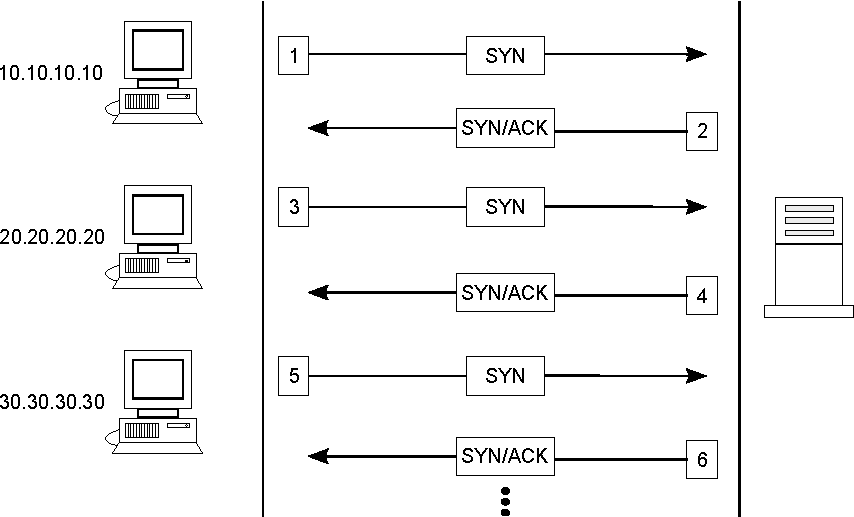
\includegraphics[width=12cm]{pics/synflood.pdf}
\caption{SYN-hyökkäys käyttäen useampaa konetta}
\label{syn}
\end{figure}

SYN-hukuttamisen mahdollistavan mekanismin avulla voidaan myös toteuttaa
heijastettu hyökkäys (engl. reflective attack), joka on muunnos SYN-
hukuttamisesta. Tässä hyökkäyksessä väärennetyissä SYN-viesteissä on
lähettäjäksi merkitty haluttu kohde. Lähettämällä suuri määrä näitä SYN-
viestejä esimerkiksi web-palvelimelle, aiheutuu vastaustulvasta ongelmia
kohteelle \cite{STACK}.

Koska harvalla yrityksellä on mahdollista pitää ylimääräisiä resursseja SYN-
hukuttamisen varalta, joudutaan ratkaisua hakemaan muilla tavoin. Yksi
alkeellinen keino on rajoittaa puoliavonaisten yhteyksien määrää, jolloin rajan
ylittyessä yhteyksiä aletaan pudottamaan \cite{TCP}. Toinen käytetty keino on
reitittimiltä verkkoon päin tulevan liikennemäärän seuraaminen, ja
liikennepiikkeihin reagoiminen. Hyökkäyksiä vastaan voidaan myös suojautua
liikenteen seuraamiseen tarkoitetuilla sovelluksilla sekä pääsylistoilla \cite{STACK}.
Täydellistä turvaa nämä eivät kuitenkaan tarjoa, sillä hyvin toteutettua
hyökkäystä on vaikea torjua.

\subsection{UDP Echo}

Myös UDP-protokolla mahdollistaa hyökkäysten tekemisen. Nämä
hyökkäykset käyt\-tä\-vät hyväkseen UDP:n ECHO-toimintaa, jos sen käyttö
on vain sallittu verkossa. Näistä hyökkäyksistä tunnetuin on Fraggleksi
nimetty hyökkäys, joka nykyisinkin aiheuttaa väärin konfiguroidussa verkossa isoja ongelmia.
Fraggle toimii siten, että hyökkääjä lähettää UDP echo-viestin yleislähetyksenä, johon on merkitty lähettäjäksi
hyökkäyksen kohde. Tähän viestiin kaikki verkon koneet pyrkivät vastaamaan,
jolloin kohdekoneen kaista ja resurssit joudutaan varaamaan viestien vastaanottamiseen (kuva \ref{echo}). 
Fraggle on hyvä esimerkki vahvistetusta hyökkäyksestä, jossa verkon laitteiden määrä
vaikuttaa siihen, kuinka vakava hyökkäys on \cite{WEBS}. Vastaavanlainen
hyökkäys voidaan myös toteuttaa kahden koneen välillä, jos kummassakin
on sallittuna UDP ECHO-viestit. Tällöin hyökkääjä väärentää viestiin
lähettäjän osoitteen ja halutun kohdeportin. Vastaanottaja vastaa
tähän viestiin omalla echo-viestillä, ja näin kahden koneen välille on
muodostunut ikuinen silmukka \cite{TCP}.

\begin{figure}[htp]
\centering
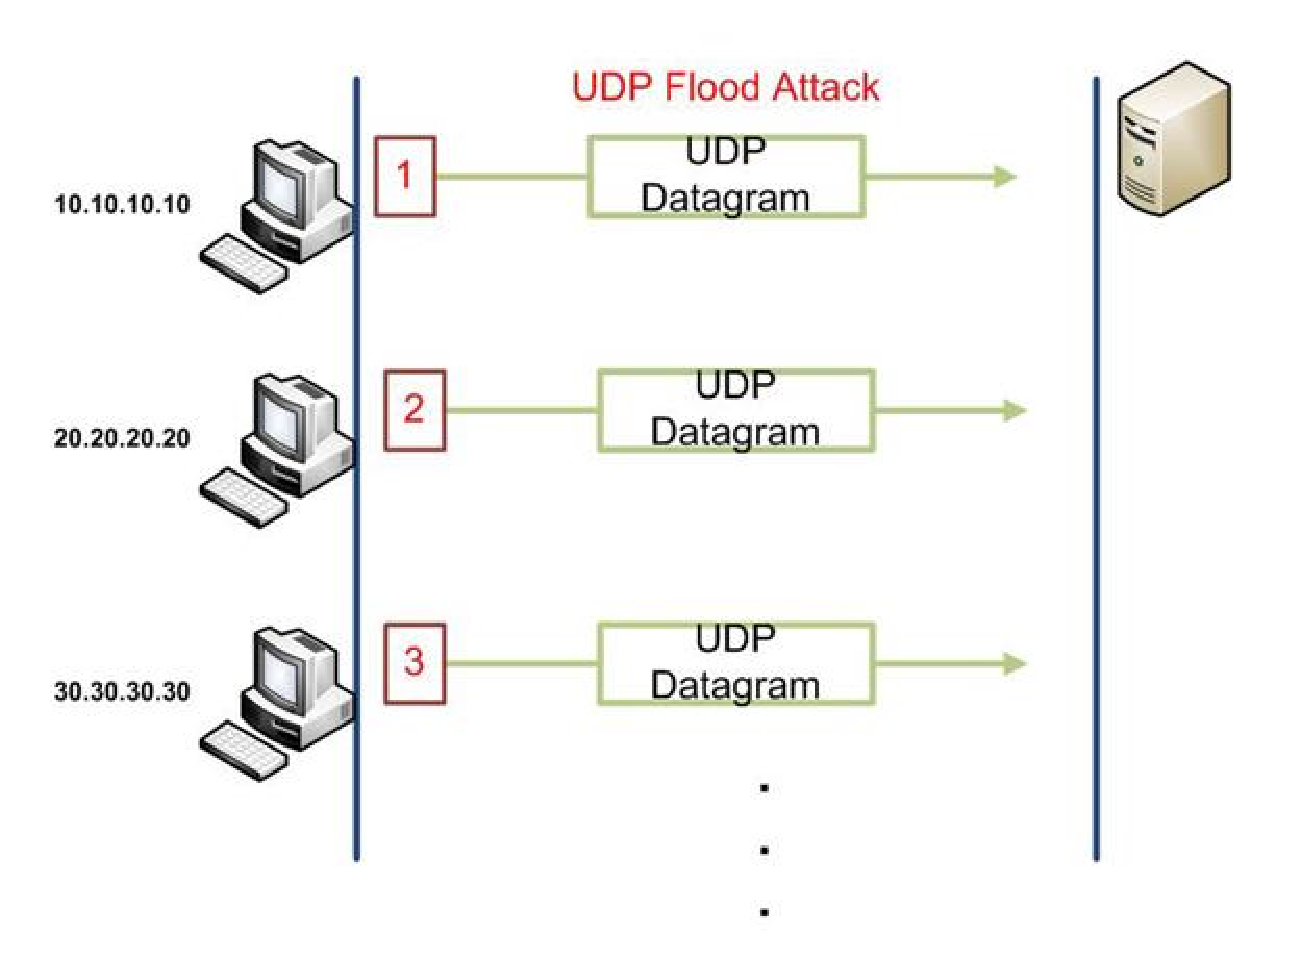
\includegraphics[width=12cm]{pics/echo.pdf}
\caption{UDP Echo hyökkäys}
\label{echo}
\end{figure}

\subsection{Smurf}

Smurf on yksi ensimmäisistä vahvistetuista DoS-hyökkäyksistä, ja se
toimii lähes identtisesti Fragglen kanssa sillä erolla, että UDP:n
sijasta käytetään ICMP-pro\-to\-kol\-laa. Hyökkääjä lähettää kohteen
puolesta yleislähetyksenä verkolle ICMP ECHO-paketin, johon verkon
laitteet vastaavat, jos ECHO-viestit on sallittuja verkossa. Jo 100
konetta verkossa pystyy aiheuttamaan 14Mbps kuorman kohdekoneelle,
joten pienikin väärin konfiguroitu verkko pystyy aiheuttamaan kuorman,
jota harva linkki pystyy pitkään kestämään \cite{Hacking}.

Jos hyökkäys on päässyt käyntiin, ei tälle ole paljoa muuta tehtävissä
kuin poistaa kohteena olevat koneet pois verkosta. Paras vastatoimi
Fragglen ja Smurffin kaltaisille hyökkäyksille onkin konfiguroida
verkon laitteet alusta asti oikein. Yleislähetysten kieltämisellä ja
ECHO-viestien tuen poistamisella verkon laitteilta pääsee jo
pitkälle. Samoin ICMP-protokollan käyttöä kannattaa verkossa rajoittaa
\cite{Hacking}.

\section{Distributed Denial of Service}

Vielä viime vuosikymmenellä palvelunestohyökkäykset perustuivat yleensä
käyttöjärjestelmistä löydettyjen heikkouksien hyödyntämiseen. Näiden
hyökkäysten aikaansaama tuho oli usein konekohtaista ja melko rajattua, joten
hyökkäyksiä ei nähty kovinkaan vakavana uhkana. 2000-luvulla
palvelunestohyökkäykset ovat kuitenkin kehittyneet siihen pisteeseen, että
nykyisin palvelu saattaa joutua hajautetun palvelunestohyökkäyksen (engl.
Distrubuted Denial of Service) kohteeksi, jolloin palvelua saattaa olla
lamauttamassa jopa yli 140000 saastunutta konetta. Tällaisia saastuneita
koneita kutsutaan zombeiksi, sillä näihin on murtauduttu ja asennettu
ohjelmisto, jonka avulla murtautuja pystyy hallitsemaan konetta käyttäjän
tietämättä. Zombie-verkoston ei tarvitse edes olla kovinkaan suuri
aiheuttaakseen tuhoa, sillä jo 3000 koneen verkosto, jossa jokainen kone
tuottaa 25 Kbps liikennettä, aiheuttaa yhteensä 75 Mbps kuorman verkolle \cite{Hacking}.
Palvelunestohyökkäyksen seuraamukset saattavatkin olla varautumattomalle
taholle usein katastrofaaliset, ja pahimmillaan hyökkäys saattaa pysäyttää
organisaation toiminnan useiksi päiviksi \cite{CERT}.

Hyökkäysten hajauttaminen useammalla koneelle tuo useita hyötyjä verrattuna
perinteiseen palvelunestohyökkäykseen, jossa hyökkäys toteutetaan käyttäen yhtä
konetta. Otetaan esimerkiksi vaikka web-palveluita tarjoava palvelin, jota
vastaan halutaan tehdä palvelunestohyökkäys. Tällaisella palvelimella on
käytössä huomattavasti suurempi määrä resursseja (kaista, muisti,
prosessointiteho) kuin mitä yhdellä tavallisella koneella on. Tekemällä
hyökkäyksen yhtäaikaisesti useammalla koneella, pystyy hakkeri kuluttamaan
suuretkin resurssit loppuun melko lyhyessä ajassa. Yhdeltä koneelta tuleva
palvelunestohyökkäys on myös helppo tunnistaa ja estää verkon ylläpitäjän
toimesta. Hyökkääjien määrän kasvaessa tehtävä vaikeutuu huomattavasti, koska
suurin osa koneista pitää tunnistaa ja liikennöinti pysäyttää, jotta tästä olisi
jonkinlaista hyötyä. Jos nämä koneet ovat vielä levitetty ympäri internetiä, on
hyökkäysten pysäyttäminen ilman palvelun kärsimistä mahdoton tehtävä käsin
tehtynä. Tällaista hyökkäysliikennettä on vaikea erottaa tavallisesta
liikenteestä, koska se tulee palvelimelle eri reittejä pitkin \cite{DDOS}.

Nopeiden yhteyksien ja verkossa olevien koneiden räjähdysmäinen kasvu on tehnyt
hajautetuista palvelunestohyökkäyksistä hyvin tehokkaita ja tuhoisia. Suuri
määrä verkossa kiinni olevista koneista on huonosti suojattu ja päivitetty, ja
ihmisten tietoisuus verkon vaaroista on usein puutteellista. Tämä on luonut
otollisen maaperän suurten zombie-verkostojen muodostamiselle virusten ja
matojen avustuksella. Tarjolla on myös tätä tarkoitusta varten suunniteltuja
työkaluja ja ohjelmistoja, jotka tekevät tarvittavat toimenpiteet
automaattisesti. Jo ensimmäiset työkalut kuten Trinoo ja Shaft, jotka ovat
vapaasti saatavilla verkosta, mahdollistivat tuhansien suojaamattomien koneiden
haltuunoton vaatimatta sen suurempaa tietämystä \cite{DDOS}.

Hyökkäyksessä käytetyt koneet voidaan jakaa agentteihin (engl. agents) ja
liikenteen ohjaajiin (engl. handlers) riippuen näiden rooleista. Näistä
koneista hyökkääjä käskyttää suoraan liikenteen ohjaajia, jotka sitten ohjaavat
annetut käskyt agenteille hyökkäyksen alettua \cite{WEBS}\cite{DDOS}. Ensimmäisissä DDoS-
verkoissa nämä ohjausviestit olivat salaamattomia, ja kuka tahansa pystyi
kaappaamaan niitä. Tämä oli ongelmallista, koska liikenteen ohjaajat joutuivat
pitämään yllä IP-listaa agenteista, jolloin liikenteen välittäjän joutuessa
vastahyökkäyksen kohteeksi, paljastui verkon jokainen kone. Tätä suoran
käskyttämisen heikkoutta pyrittiin korjaamaan mm. salaamalla liikenne ja
viestit. Ajan saatossa liikenteen ohjaajat pystyttiin kuitenkin tunnistamaan ja
poistamaan verkosta, jolloin hyökkäyksessä käytetty verkko hajosi \cite{DDOS}.

\begin{figure}[htp]
\centering
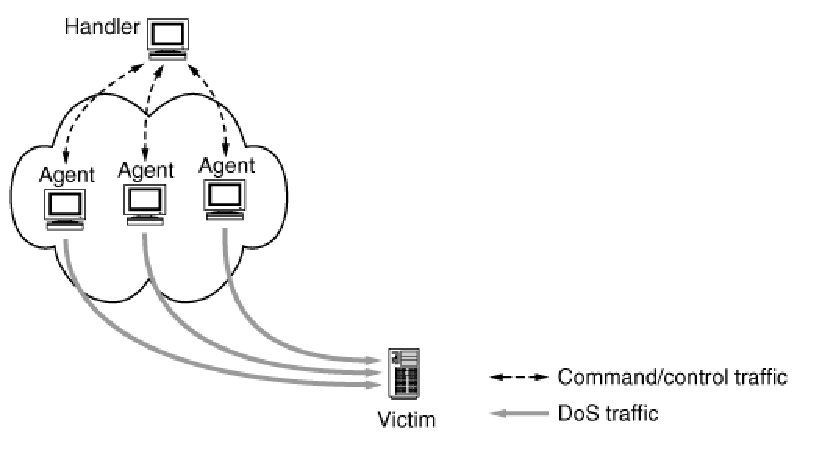
\includegraphics[width=12cm]{pics/ddos1.pdf}
\caption{Perinteinen DDoS-verkosto}
\label{ddos1}
\end{figure}

Nykyisin enää harva DDoS-hyökkäyksessä käytetty verkko käyttää kuvan \ref{ddos1}
hierarkiaa sen heikon ohjattavuuden takia. Tämän tilalle on tullut
epäsuoraan käskyttämiseen perustuvat verkot, jotka käyttävät viestien
välittämiseen IRC-verkkoja (kuva \ref{ddos2}). IRC on reaaliaikaiseen viestittämiseen
tarkoitettu palvelu, jonka kautta ihmiset pystyvät reaaliajassa kirjoittamaan
ja lukemaan viestejä. IRC-verkot muodostuvat IRC-kanavista, joita on lukematon
määrä, ja joihin käyttäjät liittyvät ennen kommunikointia. Samalla
periaatteella toimivat myös saastuneet koneet. Jokainen kone liittyy usein
salasanalla suojattuun IRC-kanavaan, jonka kautta hyökkääjä antaa käskyjä
koneille. Tällä tavalla saadaan monia etuja verrattaessa suoraan käskyttämiseen.
Ensinnäkin liikennettä ei pystytä enää tunnistamaan poikkeavaksi, koska se on
normaalia IRC-liikennettä. Toisekseen käytettyä kanavaa voidaan vaihtaa
lennosta, jolloin yhden kanavan sulkeminen ei pysäytä verkon toimintaa. Näiden
syiden takia DDoS-hyökkäysten pysäyttäminen ennen niiden käynnistymistä on
erittäin vaikeaa \cite{DDOS}.

\begin{figure}[htp]
\centering
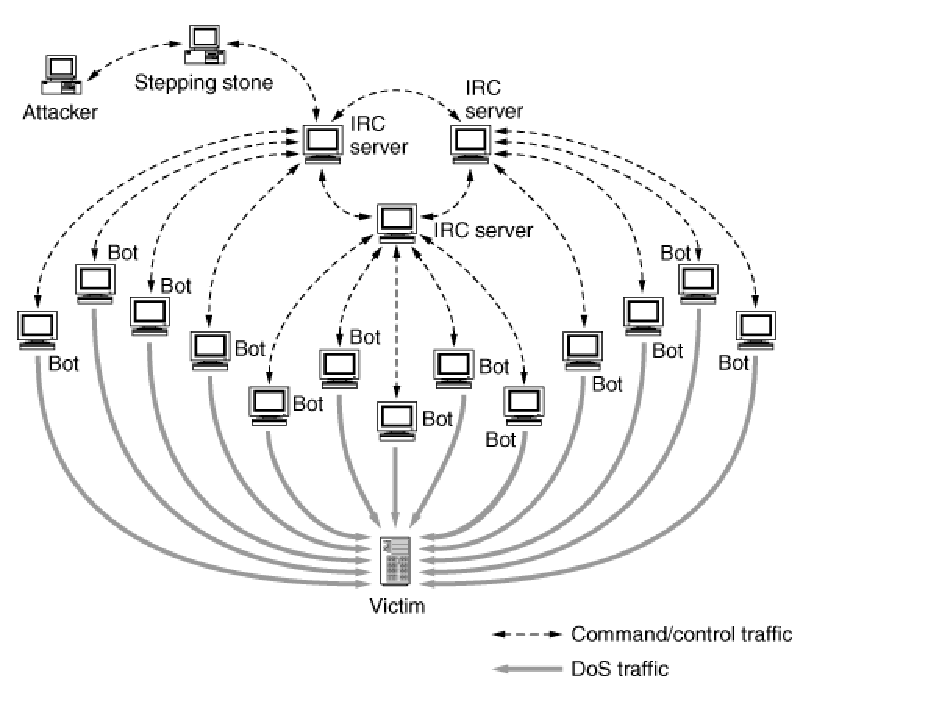
\includegraphics[width=12cm]{pics/ddos2.pdf}
\caption{Nykyaikainen DDoS-verkosto}
\label{ddos2}
\end{figure}

Kuten yllä on jo tullut esille, on hajautetulta palvelunestohyökkäykseltä
suojautuminen vaikea tehtävä riippumatta siitä onko verkko itse kohde vai
käytetäänkö sitä vain hyökkäysten koordinointiin. Valmista ja yksityiskohtaista
ratkaisua ei ole tarjolla, mutta seuraamalla joitakin yleisiä strategioita,
voidaan vahinkoja rajoittaa. Nämä strategiat ovat suojautuminen, tunnistaminen
ja reagoiminen, ja ne noudattavat yleistä vahinkoketjun elinkaarta \cite{DDOS}.

Ensinnäkin on tärkeää, että verkon ylläpitäjä tietää tarkoin kuinka verkko
toimii, ja käytössä on verkon toimintaa seuraavia työkaluja. Näiden avulla
verkon heikot kohdat pystytään tunnistamaan ja vahvistamaan. Käytössä tulee
olla myös jonkinlainen suojausjärjestelmä, joka kirjaa ylös riittävän pitkältä
ajalta ylös verkkoon tulevan ja lähtevän liikenteen, sillä aina hajautettu
palvelunestohyökkäys ei kaada koko verkkoa. Tällöin on tärkeää, että tapahtunut
pystytään tarkasti analysoimaan, ja löydetyt heikkoudet paikattua parhaalla
mahdollisella tavalla \cite{DDOS}.

Kun hyökkäys on päällä, tulee käytetty hyökkäystapa tunnistaa mahdollisimman
nopeasti. Useimmat hyökkäykset noudattavat tiettyä kaavaa, ja näiden
tunnistamiseen on olemassa useita valmiita työkaluja. Tämä on tärkeää, koska
tunnistamisen jälkeen voidaan rajata, mistä hyökkäys on peräisin ja tehdä
tarvittavat toimenpiteet hyökkäyksen torjumiseksi. Useimmissa tapauksissa
tämä tarkoittaa yhteistyötä palveluntarjoajan ja viranomaisten kanssa.
Viranomaisten mukaan tuominen on muutenkin tärkeää, koska vain tätä kautta
voidaan käytettyä hyökkäysverkostoa lähteä tunnistamaan ja toivottavasti myös
hajottamaan \cite{DDOS}.

Jotta nopea reagoiminen olisi mahdollista, tulee yrityksessä olla tehtynä
toimintasuunnitelmat hyökkäyksen varalta. Ensimmäinen vaihtoehto lienee aina
haitallisen liikenteen estäminen, mutta tätä varten tulee olla tehtynä tarkat
prosessit kuinka toimitaan hyökkäyksen alettua. Tärkeää on sopia mitä
dokumentoidaan ja kuinka asioista raportoidaan oikeille tahoille. Hyökkäyksen
jälkeinen analyysi on myös riippuvainen sovituista käytännöistä. Tämä analyysi
on erittäin tärkeää, sillä vain sitä kautta toimintasuunnitelmia voidaan
kehittää oikeaan suuntaan \cite{DDOS}.


\section{Remote-to-Local}

Remote-to-Local (lyh. R2L) on hyökkäystyyppi, jossa hyökkääjä pyrkii
saamaan koneelle sellaiset oikeudet, joita hänellä ei muuten
olisi. Tämä tapahtuu useimmiten käyttäen hyväksi järjestelmässä olevia
heikkouksia, joiden avulla hyökkääjä pääsee verkon yli murtautumaan
koneelle \cite{IDS}. Pahimmassa tapauksessa hyökkääjä saa hankittua koneelle
pääkäyttäjän oikeudet, jolloin koneen ja verkon resurssit ovat täysin
hyökkääjän käytössä.

Onnistuneet R2L hyökkäykset ovat verkon ylläpitäjien kannalta pahimpia
mahdollisia, sillä niiden mahdollistamat tuhot ja aiheuttamat kustannukset ovat
muita hyökkäyksiä huomattavasti suuremmat \cite{IDSb}. Onnistunut R2L-hyökkäys saattaa
myös muut verkon koneet vaaraan, sillä usein hyökkääjä pyrkii asentamaan
koneisiin ohjelmistoja, joiden avulla hyökkääjä pystyy ottamaan koneen haltuun
käyttäjän huomaamatta. Tällä tavoin osa aikaisemmin mainituista Zombie-
verkostoista saa alkunsa.

Käytetyimmät web-palvelinohjelmistot (Apache ja IIS) vastaavat noin 85\%
kaikista käytetyistä palvelinsovelluksista. Näiden kahden lisäksi BIND-
nimipalvelinohjelmistolla on markkinaenemmistö. Ohjelmistojen yleisyydestä
johtuen yli puolet R2L-hyökkäyksen mahdollistavista heikkouksista onkin
löydetty näille alustoille \cite{IDS}. Useat haavoittuvaisuudet johtuvat
ohjelmointivirheistä, joiden johdosta hyökkääjä pystyy aiheuttamaan
sovellukseen muistin ylivuodon (engl. Buffer Overflow). Tämä usein kaataa
sovelluksen tai saattaa sen sellaiseen tilaan, että hyökkääjä pystyy ajamaan
omia komentoja koneella. Kattava listaus löydetyistä heikkouksista ja näiden
korjauksista löytyy osoitteesta www.cve.mitre.org/cve \cite{CVE}.

Tunnetuilta R2L-hyökkäyksiltä suojautuminen on hyvin yksinkertaista sillä
nykyinen trendi on, että haavoittuvuuden löytänyt taho ilmoittaa tästä ensin
sovelluksen kehittäjille, ennen kuin julkistaa tiedon. Siksi usein korjaus
haavoittuvuuteen on olemassa ennen kuin sitä on mahdollista hyödyntää \cite{IDSb}.
Vastuu jääkin verkon ylläpitäjälle, että pitää käytetyt sovellukset ajan
tasalla sekä päivittää suojausjärjestelmät siten, että ne tunnistavat tällaiset
hyökkäykset. Suurin osa onnistuneista hyökkäyksistä johtuukin siitä, että
tunnettuja tietoturva-aukkoja ei ole korjattu.

\section{User-to-Root}

User-to-Root (lyh. U2R) hyökkäyksessä murtautuja pyrkii hankkimaan
koneelle pääkäyttäjän oikeudet. Tämä tapahtuu käyttäen järjestelmässä
olevia haavoittuvaisuuksia, joita ei ole paikattu. Useimmiten
hyökkäykset pohjautuvat koodausvirheisiin, jotka mahdollistavat
ylivuodon aiheuttamisen sekä odottamattomien syötteiden antamisen
\cite{IDS}. Käyttäjästä pääkäyttäjäksi hyökkäys eroaa R2L hyökkäyksestä
siten, että hyökkääjällä on jo valmiiksi pääsy koneelle normaalina
käyttäjänä.

U2R-hyökkäykset ovat L2R-hyökkäysten ohella vaikeimpia torjua, jos kohteena
oleva järjestelmä mahdollistaa näiden toteuttamisen. Tämä johtuu siitä, että
usein hyökkäyksestä aiheutuva liikenne muistuttaa hyvin paljon normaalia
liikennettä, jonka johdosta itsestään oppivat puolustusjärjestelmät eivät pysty
riittävän tarkasti erottamaan haitallista liikennettä normaalista \cite{U2R}.
Kehittyneimmilläkin järjestelmillä näiden hyökkäysten tunnistaminen on todella
heikkoa. Tämän on osoittanut useat eri tutkimushankkeet, jotka ovat käyttäneet
järjestelmiensä testaamiseen DARPAn simuloimaa verkkoliikennettä, jonka sisältö
on tarkkaan tiedossa. Parhaimmillaankin tunnistaminen on jäänyt 20 prosentin
paikkeille, ja yleensä luku on jäänyt alle 10 prosenttiin.
